\documentclass{article}
\usepackage[utf8]{inputenc}
\usepackage{tikz}
\usepackage{graphicx}
\graphicspath{ {./images/} }


\title{CS132 Quizzes - Assembler}
\begin{document}
\begin{center}
    \Huge\textbf{CS132 Quizzes - Assembler}\\
    \huge\textit{May 2021}\\
    \medskip
    \Large\textit{Edmund Goodman}
\end{center}


\section{Explain the role of the Arithmetic Logic Unit (ALU) in the operations
of a microprocessor}

The Arithmetic Logic Unit is a subcomponent of the microprocessor which performs
mathematical and logical operations on data within the microprocessor.

It is capable of performing various different operation, which can be selected
between by control lines, and is distinct from other components which read and
write the data to provide its inputs and store its outputs, only handling
performing the operations on the data



\section{Explain the role of the Control Unit (CU) in the operation of a
microprocessor}

The control unit is a subcomponent of the microprocessor decodes program
instructions into a set of signals which cause and control the logistics for the
execution of the instruction. For example, some signals it outputs are

It operates at the clock speed of the processor, and is dependent on the state
of other items in the microprocessor (e.g. the CCR)



\section{Outline the Fetch-Execute cycle, making reference to the role it plays
in the execution of computer programs}

The fetch-execute cycle is the sequence of steps taken by the computer to enact
a single instruction of machine code (essentially one line of assembly) stored
in memory. These steps are:

\begin{enumerate}
\item
  Fetch
  \begin{enumerate}
  \item
    Retrieve the instruction the main store (MS) at the address currently in the
    program counter (PC)
  \item
    Store the retrieved instruction in the instruction register (IR)
  \item
    Increment the program counter (PC)
  \end{enumerate}
\item
  Decode
  \begin{enumerate}
  \item
    The control unit extracts and decodes the opcode from the instruction in the
    instruction register (IR)
  \item
    Read the effective address to establish opcode type, determining whether
    another read operation is needed
  \end{enumerate}
\item
  Execute
  \begin{enumerate}
  \item
    Control unit outputs signals to control the logistics of executing the
    instruction
  \item
    Changes in the state resulting from the execution of the instruction may
    occur
  \end{enumerate}
\end{enumerate}

Computer programs, irrespective of what language they are written in, are
reduced down to a large sequence of these instructions to be run in sequence, so
the fetch-execute cycle is run many times, once for each instruction, to execute
the program



\section{Explain the role of Program Counter (PC) and Instruction Register (IR)
in the Fetch-Execute cycle}

The program counter is use to keep track of which instruction is next to be
executed in the fetch-execute cycle, ensuring the instructions are evaluated in
the correct order. In every cycle, it is incremented after the instruction is
fetched, so it points to the address of the instruction to be fetched in the
next cycle. It can also be moved by jump instructions, to allow control flow.

The instruction register stores the instruction after it is read from the
location in the main store indicated by the program counter. This copying is
important, as it means it can be accessed quickly, instead of slower operations
of reading the main store, and that in indirect addressing, it is not
overwritten by the data retrieved that is needed to perform the instruction



\section{Explain the purpose of the Condition Code Register (CCR), giving an
example of a situation in which it is used}

The condition control register is a subset of the status register within the
microprocessor, specifically those relating to the condition of the arithmetic
logic unit after the execution of an operation.

One of the ways it may be used is to indicate to the control unit that an
overflow has occurred in an arithmetic operation on two data values



\section{With the aid of a diagram, explain the role of a Compiler in process by
which machine code is generated from a high-level computer program}

The compiler takes program code written in a high level language, such as C or
Rust, and translates it into a sequence of low-level assembly instructions.
Then, an assembler is used to convert these instructions into machine code.
Whilst it does not fully convert between program code and machine code, it
performs the majority of the translation, as assembly has mostly a one-to-one
mapping with machine code

\begin{figure}
\centering
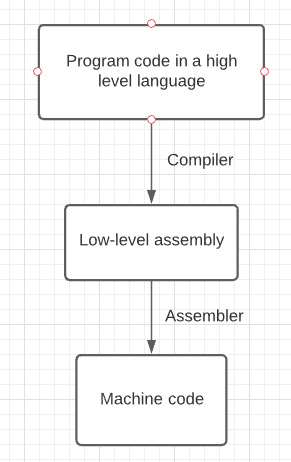
\includegraphics{compilerDiagram.png}
\caption{Compiler diagram}
\end{figure}



\section{Show the general form of a statement in assembler, giving a example of
a specific statement and showing how it related to this general form}

The general form of an instruction is as follows:

\begin{verbatim}
<opcode> <address_1> <address_2> | Comment (optional) 
\end{verbatim}

The opcode indicates what the instruction does, the addresses indicate what the
instruction should be performed on, and the optional comment indicates what the
instruction is being used for

A specific instruction, with the opcode indicating adding, and the registers
being D0 and D1 might be:

\begin{verbatim}
add.l D0, D1 | Add the value of the D1 register to the D0 register
\end{verbatim}



\section{Give an example of an arithmetic instruction in assembler \emph{(not
entirely sure if this is correct)}}
\begin{verbatim}
add.l D0, D1 | Add the value of the D1 register to the D0 register
\end{verbatim}
Using direct addressing on a long word, add the value of the D1 register to the
D0 register



\section{Explain immediate addressing, giving an example of an instruction that
uses this addressing mode}

Immediate addressing is when the actual value to be used is stored as a fixed
value within the instruction. For example, an instruction to always add a
constant number to a register might be as follows:

\begin{verbatim}
add.l D0,#$42 | Add the hexadecimal value 42 to the register D0
\end{verbatim}



\section{Explain absolute addressing, giving an example of an instruction that
uses this addressing mode and showing one disadvantage of absolute addressing}

Absolute addressing is when the actual address of the value to retrieve from the
main store memory is stored as a fixed value within the instruction. For
example, an instruction to always add the value stored at a fixed address to a
register might be as follows:

\begin{verbatim}
add.l D0, $FFF00 | Add the value at the address FFF00 in the
                   main store to the register D0
\end{verbatim}

This has the disadvantage of the fact the most programs are placed in different
places in memory at each run-time, dependent on what other programs the computer
is performing at the same time. Hence, absolute addressing is unlikely to point
to data within the remit of the program, so is not useful



\end{document}
